\documentclass[../main.tex]{subfiles}

\begin{document}
	\section{Gradino}
		\begin{figure}[h!]
			\centering
			\begin{subfigure}{0.4\textwidth}
				\[
					\gr = 
					\begin{cases}
						0 \quad t<0\\
						1 \quad t \geq 0
					\end{cases}
				\]
			\end{subfigure}
			\begin{subfigure}{0.4\textwidth}
				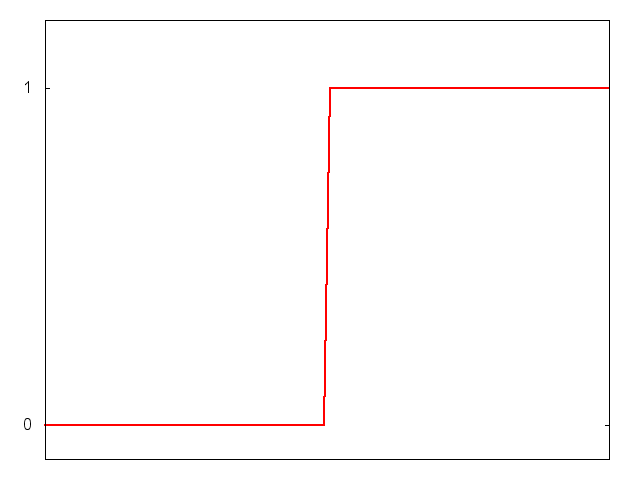
\includegraphics[width=5cm, height=3cm]{funzioni_generalizzate/gradino}
			\end{subfigure}
		\end{figure}
		Presenta una discontinuità in $t=0$.
		
	\section{Rampa}
		\begin{figure}[h!]
			\centering
			\begin{subfigure}{0.4\textwidth}
				\[
					ram(t)= t \cdot \gr =
					\begin{cases}
						0 \quad t<0\\
						t \quad t \geq 0			
					\end{cases}
				\]
			\end{subfigure}
			\begin{subfigure}{0.4\textwidth}
				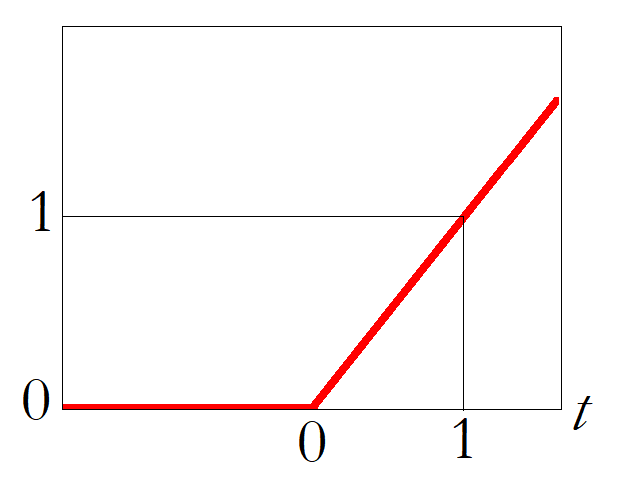
\includegraphics[width=5cm, height=3cm]{funzioni_generalizzate/rampa}
			\end{subfigure}
		\end{figure}
		In $t=0$ \'e continua, ma presenta una discontinuit\'a di prima specie nella derivata.
		
	\section{Parabola}
		\begin{figure}[h!]
			\centering
			\begin{subfigure}{0.4\textwidth}
				\[
					par(t)= ram(t) \cdot \gr = 
					\begin{cases}
						0 \quad &t<0\\
						\frac{t^2}{2} \quad &t\geq 0
					\end{cases}
				\]
			\end{subfigure}
			\begin{subfigure}{0.4\textwidth}
				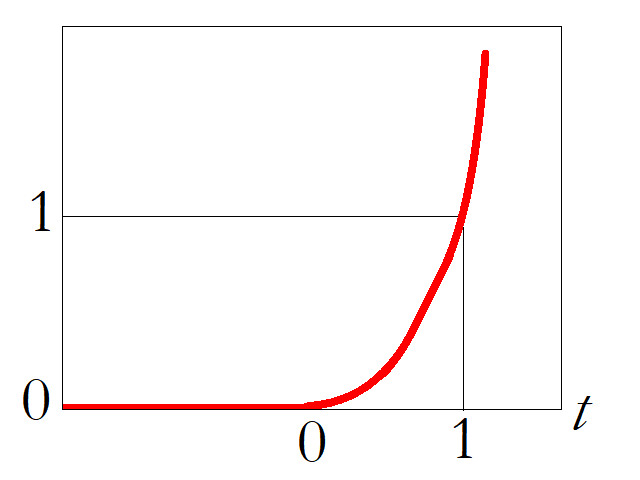
\includegraphics[width=5cm, height=3cm]{funzioni_generalizzate/parabola}
			\end{subfigure}
		\end{figure}
		Risulta continua e con derivata continua anche in $t=0$.	
		
	\section{Polinomio di grado n}
		\[
			pol(t)=\frac{t^n}{n} \cdot \gr =
			\begin{cases}
				0 \quad &t<0\\
				\frac{t^n}{n} \quad &t\geq 0
			\end{cases}
		\]
		
	\section{Derivate e integrali delle funzioni generalizzate}
		\begin{align*}
			&ram(t) = \int_{- \infty}^{t} \gr[\tau] \mathrm{d}\tau &&\der{}{t} ram(t) = \gr\\
			&par(t) = \int_{- \infty}^{t} ram(\tau) \mathrm{d} \tau &&\der{}{t} par(t) = ram(t)	
		\end{align*}
		
	\section{Impulso}
		Introduco la funzione $ \textbf{1}_{\Delta}(t) $ definita come:
		\[
			\int_{- \infty}^{t} \der{}{t}1_{\Delta}(t) \mathrm{d}\tau=
			\begin{cases}
				1 \quad t>\Delta\\
				0 \quad t<0
			\end{cases}
		\]
		Non consideriamo il caso in cui $0<t<\Delta$.\\
		\linebreak
		Definisco $\delta(t)$ la funzione $\der{}{t}1_{\Delta}(t)$ quando $\Delta \longrightarrow 0$. Valgono dunque le seguenti relazioni: 
		\begin{figure}[h!]
			\centering
			\begin{subfigure}{0.5\textwidth}
				\[
				\int_{-t}^{t} \delta(\tau) \mathrm{d}\tau =1 \quad \forall t>0, \qquad \der{}{t} \gr = \delta(t)
				\]
			\end{subfigure}
			\begin{subfigure}{0.4\textwidth}
				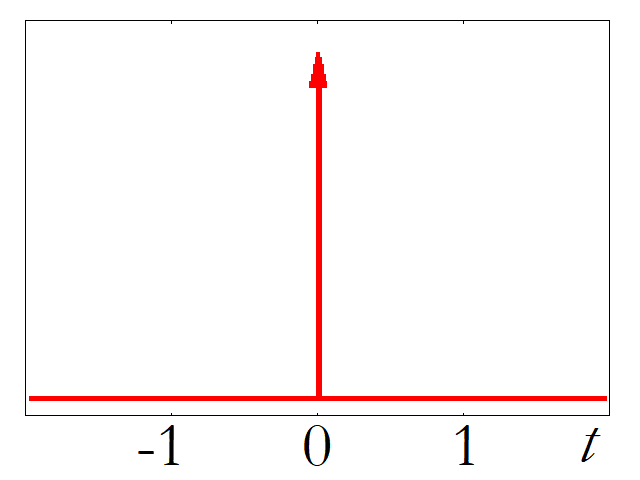
\includegraphics[width=5cm, height=3cm]{funzioni_generalizzate/impulso}
			\end{subfigure}
		\end{figure}
		%
		\linebreak
		L'impulso \'e caratterizzato dal valore della sua area, determinato dal coefficiente della funzione.\\
		%grafico
		\linebreak
		L'impulso torna utile quando bisogna effettuare il \textbf{campionamento} di una funzione, cio\'e determinare il valore della funzione nel punto in cui viene applicato l'impulso.
		\begin{align*}
			f(t)\ \delta(t) &= f(0)\ \delta(t)\\
			f(t)\ \delta(t - T) &= f(T)\ \delta(t - T)   
		\end{align*}
		
	\section{Doppietto}
		Derivando ulteriormente $\der{}{t}1_{\Delta}(t)$ in un intorno $I(0)$ e in $I(\Delta)$ si ottengo due impulsi unitari: il primo centrato nell'origine, mentre il secondo centrato in $\Delta$ e negativo.\\
		Per $\Delta \longrightarrow 0$ si ottiene:
		\begin{figure}[h!]
			\centering
			\begin{subfigure}{0.5\textwidth}
				\[
					\der{}{t} \delta(t) = \dot{\delta}(t)
				\]
			\end{subfigure}
			\begin{subfigure}{0.4\textwidth}
				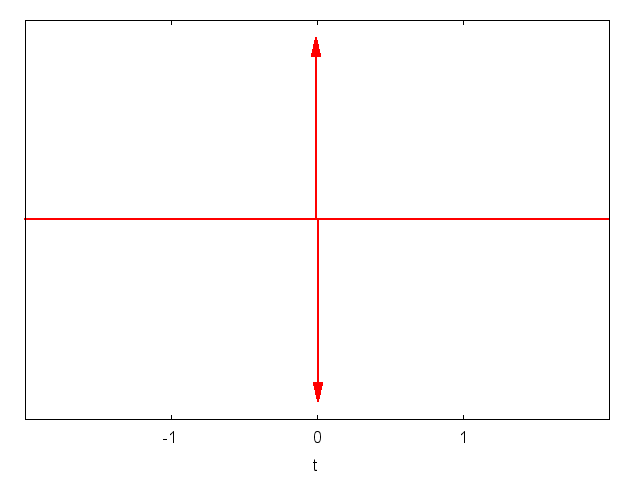
\includegraphics[width=5cm, height=3cm]{funzioni_generalizzate/doppietto}
			\end{subfigure}
		\end{figure}
		\newpage
		
	\section{Riepilogo}
		\[
			par(t) \quad \stackrel[\int_{-\infty}^{t}]{\der{}{t}}{\rightleftharpoons} 
			\quad ram(t) \quad
			\stackrel[\int_{-\infty}^{t}]{\der{}{t}}{\rightleftharpoons}
			\quad \gr \quad
			\stackrel[\int_{-\infty}^{t}]{\der{}{t}}{\rightleftharpoons}
			\quad \delta (t) \quad
			\stackrel[\int_{-\infty}^{t}]{\der{}{t}}{\rightleftharpoons}
			\quad \dot{\delta}(t) \quad
		\]
		
	\section{Trasformazioni delle funzioni}
	
	\subsection{Traslazione}
		$$ f(x) = f(x - t) $$
		\begin{itemize}
			\item $ t>0 $: ritardo, la funzione è traslata verso dx di t
			\item $ t<0 $: anticipo, la funzione è traslata verso sx di t 	
		\end{itemize}
		
	\subsection{Scalamento}
		$$ f(x) = f(x \cdot t) $$
		\begin{itemize}
			\item $ 0<t<1 $: la funzione si estende di un fattore t
			\item $ t>1 $: la funzione viene compressa di un fattore t  	
		\end{itemize}
		
	\subsection{Simmetrie}
		\begin{itemize}
			\item $ f(x) = f(-x) $: simmetrica rispetto l'asse delle y
			\item $ f(x) = -f(x) $: simmetrica rispetto l'asse delle x  	
		\end{itemize}
		%
	\section{Rettangolo}
		%grafico
		$$ R_{t_{1},t_{2}}(t) = \gr[t - t_{1}] - \gr[t - t_{2}] $$
		
	\begin{Exercise}[title={Derivata di una funzione definita a tratti}, difficulty=3]
		Dividiamo il grafico \ref{fig:grafico_f} in sezioni e per ognuna scriviamo la funzione 'finestrata' (cioè moltiplicata per un rettangolo di base pari alla larghezza della sezione):
		\begin{figure}[h!]
			\centering
			\resizebox{.7\columnwidth}{!}{% GNUPLOT: LaTeX picture with Postscript
\begingroup
  \makeatletter
  \providecommand\color[2][]{%
    \GenericError{(gnuplot) \space\space\space\@spaces}{%
      Package color not loaded in conjunction with
      terminal option `colourtext'%
    }{See the gnuplot documentation for explanation.%
    }{Either use 'blacktext' in gnuplot or load the package
      color.sty in LaTeX.}%
    \renewcommand\color[2][]{}%
  }%
  \providecommand\includegraphics[2][]{%
    \GenericError{(gnuplot) \space\space\space\@spaces}{%
      Package graphicx or graphics not loaded%
    }{See the gnuplot documentation for explanation.%
    }{The gnuplot epslatex terminal needs graphicx.sty or graphics.sty.}%
    \renewcommand\includegraphics[2][]{}%
  }%
  \providecommand\rotatebox[2]{#2}%
  \@ifundefined{ifGPcolor}{%
    \newif\ifGPcolor
    \GPcolortrue
  }{}%
  \@ifundefined{ifGPblacktext}{%
    \newif\ifGPblacktext
    \GPblacktextfalse
  }{}%
  % define a \g@addto@macro without @ in the name:
  \let\gplgaddtomacro\g@addto@macro
  % define empty templates for all commands taking text:
  \gdef\gplbacktext{}%
  \gdef\gplfronttext{}%
  \makeatother
  \ifGPblacktext
    % no textcolor at all
    \def\colorrgb#1{}%
    \def\colorgray#1{}%
  \else
    % gray or color?
    \ifGPcolor
      \def\colorrgb#1{\color[rgb]{#1}}%
      \def\colorgray#1{\color[gray]{#1}}%
      \expandafter\def\csname LTw\endcsname{\color{white}}%
      \expandafter\def\csname LTb\endcsname{\color{black}}%
      \expandafter\def\csname LTa\endcsname{\color{black}}%
      \expandafter\def\csname LT0\endcsname{\color[rgb]{1,0,0}}%
      \expandafter\def\csname LT1\endcsname{\color[rgb]{0,1,0}}%
      \expandafter\def\csname LT2\endcsname{\color[rgb]{0,0,1}}%
      \expandafter\def\csname LT3\endcsname{\color[rgb]{1,0,1}}%
      \expandafter\def\csname LT4\endcsname{\color[rgb]{0,1,1}}%
      \expandafter\def\csname LT5\endcsname{\color[rgb]{1,1,0}}%
      \expandafter\def\csname LT6\endcsname{\color[rgb]{0,0,0}}%
      \expandafter\def\csname LT7\endcsname{\color[rgb]{1,0.3,0}}%
      \expandafter\def\csname LT8\endcsname{\color[rgb]{0.5,0.5,0.5}}%
    \else
      % gray
      \def\colorrgb#1{\color{black}}%
      \def\colorgray#1{\color[gray]{#1}}%
      \expandafter\def\csname LTw\endcsname{\color{white}}%
      \expandafter\def\csname LTb\endcsname{\color{black}}%
      \expandafter\def\csname LTa\endcsname{\color{black}}%
      \expandafter\def\csname LT0\endcsname{\color{black}}%
      \expandafter\def\csname LT1\endcsname{\color{black}}%
      \expandafter\def\csname LT2\endcsname{\color{black}}%
      \expandafter\def\csname LT3\endcsname{\color{black}}%
      \expandafter\def\csname LT4\endcsname{\color{black}}%
      \expandafter\def\csname LT5\endcsname{\color{black}}%
      \expandafter\def\csname LT6\endcsname{\color{black}}%
      \expandafter\def\csname LT7\endcsname{\color{black}}%
      \expandafter\def\csname LT8\endcsname{\color{black}}%
    \fi
  \fi
    \setlength{\unitlength}{0.0500bp}%
    \ifx\gptboxheight\undefined%
      \newlength{\gptboxheight}%
      \newlength{\gptboxwidth}%
      \newsavebox{\gptboxtext}%
    \fi%
    \setlength{\fboxrule}{0.5pt}%
    \setlength{\fboxsep}{1pt}%
\begin{picture}(7200.00,5040.00)%
    \gplgaddtomacro\gplbacktext{%
      \csname LTb\endcsname%
      \put(1007,264){\makebox(0,0)[r]{\strut{}$-1$}}%
      \put(1007,828){\makebox(0,0)[r]{\strut{}$-0.5$}}%
      \put(1007,1392){\makebox(0,0)[r]{\strut{}$0$}}%
      \put(1007,1956){\makebox(0,0)[r]{\strut{}$0.5$}}%
      \put(1007,2520){\makebox(0,0)[r]{\strut{}$1$}}%
      \put(1007,3083){\makebox(0,0)[r]{\strut{}$1.5$}}%
      \put(1007,3647){\makebox(0,0)[r]{\strut{}$2$}}%
      \put(1007,4211){\makebox(0,0)[r]{\strut{}$2.5$}}%
      \put(1007,4775){\makebox(0,0)[r]{\strut{}$3$}}%
      \put(330,1109){\makebox(0,0){\strut{}$-1$}}%
      \put(1139,1109){\makebox(0,0){\strut{}$0$}}%
      \put(1948,1109){\makebox(0,0){\strut{}$1$}}%
      \put(2757,1109){\makebox(0,0){\strut{}$2$}}%
      \put(3567,1109){\makebox(0,0){\strut{}$3$}}%
      \put(4376,1109){\makebox(0,0){\strut{}$4$}}%
      \put(5185,1109){\makebox(0,0){\strut{}$5$}}%
      \put(5994,1109){\makebox(0,0){\strut{}$6$}}%
      \put(6803,1109){\makebox(0,0){\strut{}$7$}}%
    }%
    \gplgaddtomacro\gplfronttext{%
    }%
    \gplbacktext
    \put(0,0){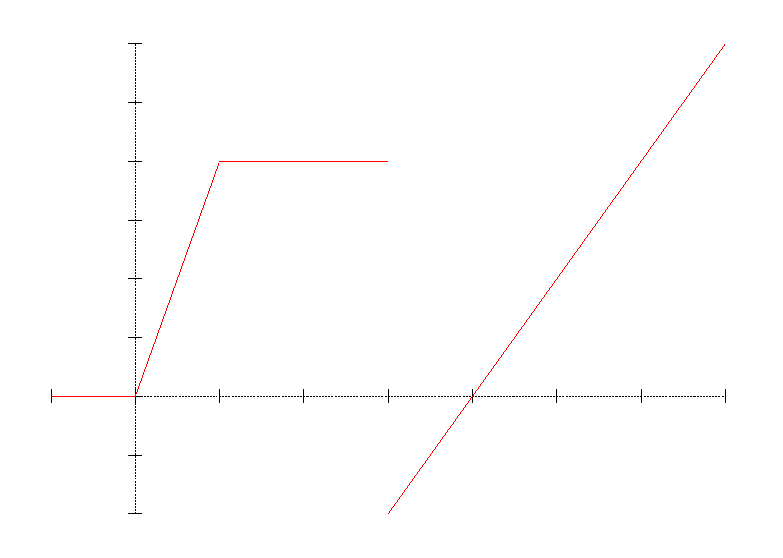
\includegraphics{funzioni_generalizzate/esercizi/derivata_funzione_def_tratti}}%
    \gplfronttext
  \end{picture}%
\endgroup
}
			\caption{Grafico di $ f(t) $}
			\label{fig:grafico_f}
		\end{figure}
		$$ f(t) = 2t \cdot R_{0,1}(t) + 2 \cdot R_{1,3}(t) + (t-4) \cdot R_{3,\infty}(t) $$
		Riscriviamo i rettangoli attraverso i gradini:
		\begin{align*}
			f(t) &= 2t \cdot \big[ \gr[t-0] - \gr[t-1] \big] &&+ 2\ \big[\gr[t-1] - \gr[t-3]\big] & +&(t-4)\ \big[\gr[t-3] - \underbrace{\gr[t - \infty]}_{0} \big] =\\
			&= 2t \cdot \gr[t] &&+ (-2t+2) \cdot \gr[t-1] & +&(-2+t-4) \cdot \gr[t-3] =\\
			&= 2t \cdot \gr[t] &&- 2(t-1) \cdot \gr[t-1] & +&(t-6) \cdot \gr[t-3]
		\end{align*}
		Quindi si pu\'o continuare in due modi equivalenti:
		\begin{enumerate}
			\item si riconducono le funzioni a funzioni generalizzate e si deriva:
				\begin{align}
					\intertext{se sostiutiamo: $ (t-6) \cdot \gr[t-3] = (t-3) \cdot \gr[t-3] - 3 \cdot \gr[t-3] = ram(t-3) - 3 \cdot \gr[t-3] $}
					f(t) &= 2 \cdot ram(t) &&- 2 \cdot ram(t-1) &&+ram(t-3) &&- 3 \cdot \gr[t-3] \nonumber\\
					\dot{f(t)} &= 2 \cdot \textbf{1}(t) &&- 2 \cdot \gr[t-1] &&+ \gr[t-3] && - 3 \cdot \delta(t-3)
					\label{derivata_es2.11.2}
				\end{align}
			\item si usano le derivate del prodotto:
			$$ \dot{f(t)} = \big[ 2 \cdot \gr[t] + 2t \cdot \delta(t) \big]\ -\ 2 \cdot \gr[t-1]\ -\ 2 \cdot (t-1) \cdot \delta(t-1)\ +\ \gr[t-3]\ +\ (t-6) \cdot \delta(t-3) $$
			Attraverso il campionamento si ha che:
			\begin{itemize}
				\item $ t \cdot \delta(t) = 0 $: campionamento in zero della retta passante per l'origine
				\item $ (t-1) \cdot \delta(t-1) = 0$: analogo al punto precedente
				\item $ (t-6) \cdot \delta(t-3) = - 3 \cdot \delta(t-3) $: la retta $ y=t-6 $ calcolata in $ t=3 $ vale -3. 
			\end{itemize}
			Dopo queste semplificazioni si ottiene l'espressione \ref{derivata_es2.11.2}.
		\end{enumerate}
	\end{Exercise}
\end{document}